\documentclass[UTF8,a4paper,10pt,fontset=fandol]{ctexart}
\usepackage[margin=13mm,top=11mm,bottom=12mm]{geometry}
\usepackage{amsmath,booktabs,graphicx,xcolor,hyperref,caption,etoolbox,tabularx,array}
\hypersetup{colorlinks=true,urlcolor=blue!55!black,linkcolor=black}
\setlength{\parindent}{2em}
\setlength{\parskip}{1.5pt}
\linespread{1.03}
\ctexset{section={format=\normalsize\bfseries,beforeskip=5pt,afterskip=2pt}}
\captionsetup{font=footnotesize,skip=2pt}
\newcolumntype{Y}{>{\raggedright\arraybackslash}X}
\newcommand{\RepoURL}{https://github.com/wszkxlllll/AI_Lab1}
\newcommand{\StudentName}{周可轩}
\newcommand{\StudentID}{10234700473}
\newcommand{\StudentInfo}{姓名：\StudentName\quad 学号：\StudentID}

\newcommand{\SelectedFone}{94.83}
\newcommand{\SelectedAccuracy}{94.84}
\newcommand{\NumberRuns}{45}


\begin{document}
\pagestyle{plain}
\fontsize{9pt}{10.5pt}\selectfont
\noindent\textbf{GitHub：}\ifdefempty{\RepoURL}
{\textcolor{red!60!black}{待填写真实仓库链接}}
{\expandafter\url\expandafter{\RepoURL}}

\begin{center}
{\Large\bfseries 实验一：新闻文本分类}\par
\vspace{1pt}
{\small 分类器、文本表示与标题信息的比较\quad\StudentInfo}
\end{center}
\vspace{-7pt}

\section{问题与实验设置}
在这个实验中，我将比较三个问题：不同分类器在同一表示下有何差异；词频加权和平均词向量是否对分类效果有帮助；标题与正文分开表示是否有收益。之后，我将进一步改变多层感知机（MLP）的容量与正则化，探索验证表现是否随训练拟合一起改善。

数据集包含 7,368 条有标签文本和 10 个类别，各类 705--747 条。采用分层 8:2 划分，随机种子设为 66；种子 88 只用于复核入选配置。主划分得到 5,894 条训练样本和 1,474 条验证样本。清洗后发现 2 条验证文本与训练内容相同，计算指标时将其排除，实际评价 1,472 条。词表、IDF 和 Word2Vec 均只在训练部分拟合，无标签测试集不参与选择。主指标为 Macro-F1，同时记录 Accuracy、各类指标和训练时间。

\section{文本表示与模型原理}
原始文本类似新闻组邮件：开头含有 \texttt{From}、\texttt{Subject}、\texttt{Organization} 等字段，空行之后才是正文。预处理只保留 \texttt{Subject} 作为标题，并保留正文；作者、组织和发帖主机等来源信息被删去，避免模型依靠来源判断类别。同一讨论的标题可能连续带有多个 \texttt{Re:}，因此也将它们去掉。

随后把英文统一转成小写，并以单词为单位统计，只保留长度不少于 2 的词；常见词没有额外删除，单复数或时态也不合并。BoW 直接记录词频，TF-IDF 则进一步降低常见词的权重、突出更有区分度的词。两者使用同一词表，最多保留 15,000 个词。\texttt{min\_df=2} 表示一个词至少出现在 2 篇训练文本中，\texttt{max\_df=0.98} 表示去掉在超过 98\% 文本中都出现、几乎没有区分度的词。最后把每篇文本的向量缩放到相同长度，避免长文本仅因词数更多而占优势：
\[
\operatorname{idf}(t)=\log\frac{1+n}{1+\operatorname{df}(t)}+1,\quad
x=\frac{\operatorname{tf}\cdot\operatorname{idf}}{\|\operatorname{tf}\cdot\operatorname{idf}\|_2}.
\]
另尝试 200 维 Skip-gram Word2Vec（窗口 5，最低词频 2，训练 20 轮），用词向量均值表示整篇文本。该表示只从训练语料学习，没有使用外部预训练权重。

\begin{center}
\footnotesize
\begin{tabularx}{\columnwidth}{@{}lY@{}}
\toprule
模型 & 原理与复杂度\\
\midrule
NB & 依据贝叶斯公式和条件独立假设累积词项证据，训练与预测都很快。\\
SVM & 在线性特征空间中寻找最大间隔超平面，$C$ 控制间隔与错分惩罚。\\
LR & 用 softmax 概率和交叉熵学习线性边界，$C$ 越大正则化越弱。\\
MLP & ReLU 隐层学习非线性组合，容量较大，但训练更慢，也更容易拟合训练噪声。\\
\bottomrule
\end{tabularx}
\end{center}

\section{训练流程与超参数搜索}
先固定文本表示，在同一训练/验证划分上比较四种模型。首轮搜索 NB 的 $\alpha\in\{0.1,1,10\}$，SVM 的 $C\in\{0.1,1,10\}$，LR 的 $C\in\{1,10,100\}$；MLP 先固定 64 个隐层单元，尝试 $\alpha\in\{10^{-4},10^{-2},1\}$。若 NB、SVM 或 LR 的最好结果落在边界，再向外补查一个数量级。MLP 使用 Adam、ReLU、学习率 0.001、批量 256，最多 300 轮；训练损失连续 15 轮没有达到 $10^{-4}$ 的改进量时停止。

确定首轮 TF-IDF 方案后，再依次改变文本结构、标题权重、MLP 宽度和层数。这样每组对照只回答一个主要问题。所有配置均保存参数、迭代次数、耗时、混淆矩阵和逐条预测，最终方案按 Macro-F1 选择。

\section{模型与表示的结果}
\begin{center}
\footnotesize
\captionof{table}{各“表示$\times$模型”的最佳验证结果。时间只计算分类器拟合。}
\resizebox{0.86\textwidth}{!}{%
\begin{tabular}{lllrrr}
\toprule
表示 & 模型 & 参数 & Acc/\% & F1/\% & 时间/s\\
\midrule
BoW & NB & $\alpha=0.01$ & 93.34 & 93.36 & 0.01 \\
BoW & SVM & $C=10$ & 90.01 & 90.01 & 14.86 \\
BoW & LR & $C=100$ & 91.44 & 91.46 & 8.02 \\
BoW & MLP & 64, $\alpha=0.0001$ & 93.95 & 93.95 & 80.51 \\
TF-IDF & NB & $\alpha=0.1$ & 93.48 & 93.51 & $<0.01$ \\
TF-IDF & SVM & $C=1$ & 93.21 & 93.23 & 18.58 \\
TF-IDF & LR & $C=100$ & 93.48 & 93.48 & 5.09 \\
TF-IDF & MLP & 64, $\alpha=0.0001$ & 94.23 & 94.22 & 99.14 \\
Word2Vec & LR & $C=10$ & 87.50 & 87.45 & 0.82
\\
\bottomrule
\end{tabular}}
\end{center}

逐步尝试后发现，TF-IDF 相对 BoW 使 SVM、LR、MLP 的最佳 F1 分别提高 3.22、2.02、0.27 个百分点，NB 也提高 0.15 个百分点。当前 TF-IDF 训练矩阵有 15,000 维，但非零元素只占 0.80\%；每篇文本通常只激活少量词项，类别又可由一组区分词形成近似线性边界。SVM 直接寻找大间隔线性边界，LR 则用正则化权重累积各词项对类别的贡献，因此都适合这种高维稀疏输入。NB 的条件独立假设虽然不完全成立，但新闻主题常由若干高区分度词共同指示；多项式 NB 可以直接累积这些非负词项证据，而较均衡的类别分布也减弱了先验偏置，因此以很小的计算量取得了 93.51\% 的 F1。MLP 的 94.22\% 最高，但拟合约需 99 秒；LR 用约 5 秒达到 93.48\%。

参数搜索也改变了比较结论。TF-IDF＋SVM 的 $C$ 从 0.1 增至 1 时，F1 从 84.72\% 升至 93.23\%，继续增至 10 反而略降；LR 的 $C=10$ 与 100 分别为 93.47\% 和 93.48\%，补查 1,000 后降至 93.35\%。平均 Word2Vec＋LR 最高为 87.45\%，词向量构造另耗时约 213 秒。这只说明当前小语料上“从头训练＋均值聚合”的效果，不代表预训练词向量或 BERT。

\newpage
\begin{center}
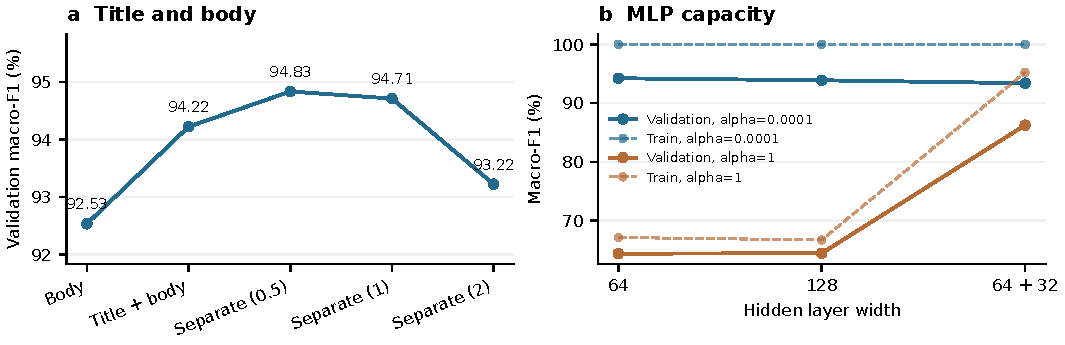
\includegraphics[width=0.94\textwidth]{figures/comparisons.pdf}
\captionof{figure}{主划分上的进一步探索。a，正文、标题正文拼接及三种标题权重；b，不同 MLP 结构在弱、强正则化下的训练与验证 Macro-F1。}
\end{center}
\vspace{-7pt}

\section{标题和正文怎样组合}
首轮比较确定分类器和参数后，继续尝试仅正文、标题正文直接拼接，以及分别做 TF-IDF 后再拼接。分开表示时，标题词表上限为 2,500，正文为 15,000；两部分先各自归一化，再按 $[\lambda\hat{x}_{\rm title};\hat{x}_{\rm body}]$ 拼接并归一化，$\lambda\in\{0.5,1,2\}$。

只保留正文时 F1 为 92.53\%，加入标题后升至 94.22\%；逐条比较中有 34 条由错变对，也有 9 条由对变错。分别表示并取 $\lambda=0.5$ 时达到 94.83\%，$\lambda=1$ 为 94.71\%，继续加到 2 则降至 93.22\%。标题确实提供了主题线索，但权重过高会压过正文信息。

种子 88 上，直接拼接和 $\lambda=0.5$ 分别得到 93.57\% 与 93.44\%，顺序与主划分相反。因此，分开表示在主划分上的 0.61 个百分点提升值得记录，却不足以说明它具有稳定优势。


这一处理会同时改变特征维数、词表和 IDF 的统计范围，因此观察到的差异属于整套结构处理，不能只归因于标题权重。这里的改进点也不是提出新算法，而是利用了数据中已有的标题结构。

\section{MLP 容量与过拟合}
在固定 TF-IDF 输入下，尝试单层 64、单层 128 和双层 64＋32，并分别设置 $\alpha=10^{-4}$ 与 1。三种结构的参数量约为 96.1 万、192.1 万和 96.2 万；64＋32 同时改变层数和参数连接方式，不能当作只改变深度的严格对照。

在 $\alpha=10^{-4}$ 时，三种结构的训练 F1 都约为 99.98\%，验证 F1 却从 64 单元的 94.22\% 依次降至 93.88\% 和 93.38\%；128 单元拟合时间还由 99 秒增至 174 秒。训练拟合继续增强并没有换来更好的泛化，表现出过拟合风险。$\alpha=1$ 时，单层 64 和 128 都只有约 64.4\%，训练分数也偏低，属于正则化过强造成的欠拟合；双层 64＋32 回升到 86.24\%。这些结果说明结构与正则化需要一起判断。


\section{分类表现与错误分析}
主划分最终选择 TF-IDF、标题正文分别表示、$\lambda=0.5$ 和 64 单元 MLP（$\alpha=10^{-4}$），Accuracy 为 \SelectedAccuracy\%，Macro-F1 为 \SelectedFone\%，共有 76 条错分。标签 2 的 F1 最低（86.90\%），标签 9 最高（98.94\%）；1$\rightarrow$2 与 2$\rightarrow$1 各有 9 例，2$\rightarrow$7 有 7 例。一个标题为 ``Laser vs Bubblejet?'' 的样本仅看正文被判为 0，加入标题后改为正确的 7，说明短标题能补充正文中不突出的主题词。


由于课程材料没有给出数字标签与新闻组名称的对应表，错误分析保留原始标签，不自行命名类别。Notebook 中给出了完整分类报告和混淆矩阵，便于继续查看具体样本。

\section{结论与局限}
综合来看，TF-IDF 在当前数据上比简单平均 Word2Vec 更有效；MLP 得到最高主划分分数，但相对 LR 的提升不到 1.4 个百分点，训练代价约高 19 倍。标题结构带来了一次小幅提升，却没有在种子 88 上复现。最终预测仍按预先确定的 Macro-F1 规则选择最高配置；若实际应用更看重速度，TF-IDF＋LR 会是更均衡的方案。


实验的结论只适用于当前语料、预处理和搜索范围。两个随机划分存在样本重叠，种子 88 也只是复核，不是独立测试集；测试集没有标签，因此不报告测试准确率。最终方案在全部 7,368 条有标签数据上重新拟合，并按原顺序生成无表头的 \texttt{prediction.csv}。

\section{复现信息}
运行环境为 Python 3.11.7、scikit-learn 1.2.2、Gensim 4.3.0 和 i9-13900H CPU。随机种子、参数范围、划分行号和逐次结果均保存在仓库；README 给出环境、运行和 XeLaTeX 编译命令。

\vspace{2pt}
{\footnotesize\noindent
参考资料：\href{https://scikit-learn.org/1.2/modules/feature_extraction.html}{[1] scikit-learn：文本表示}；
\href{https://scikit-learn.org/1.2/modules/naive_bayes.html}{[2] scikit-learn：NB}；
\href{https://scikit-learn.org/1.2/modules/svm.html}{[3] scikit-learn：SVM}；
\href{https://scikit-learn.org/1.2/modules/neural_networks_supervised.html}{[4] scikit-learn：MLP}；
\href{https://radimrehurek.com/gensim/models/word2vec.html}{[5] Gensim：Word2Vec}。}
\end{document}
